% define \title (only used by writelatex.com)
%\title{CSEC-520/620 Project Report}
%%%%%%%%%%%%%%%%%%%%%%%%%%%%%%%%%%%%%%%%%%%%%%%%%%%%%%%%%%%%%%%%%%%%%%
% LaTeX Template: Project Titlepage
%
% Source: http://www.howtotex.com
% Date: April 2011
% 
% This is a title page template which be used for articles & reports.
% 
% Feel free to distribute this example, but please keep the referral
% to howtotex.com
% 
%%%%%%%%%%%%%%%%%%%%%%%%%%%%%%%%%%%%%%%%%%%%%%%%%%%%%%%%%%%%%%%%%%%%%%
% How to use writeLaTeX: 
%
% You edit the source code here on the left, and the preview on the
% right shows you the result within a few seconds.
%
% Bookmark this page and share the URL with your co-authors. They can
% edit at the same time!
%
% You can upload figures, bibliographies, custom classes and
% styles using the files menu.
%
% If you're new to LaTeX, the wikibook is a great place to start:
% http://en.wikibooks.org/wiki/LaTeX
%
%%%%%%%%%%%%%%%%%%%%%%%%%%%%%%%%%%%%%%%%%%%%%%%%%%%%%%%%%%%%%%%%%%%%%%
%
% --------------------------------------------------------------------
% Preamble
% --------------------------------------------------------------------
%\documentclass[ fontsize=11pt,twoside]{scrartcl}	% KOMA
\documentclass[conference]{IEEEtran}
\usepackage[letterpaper,pdftex, left=.75in, right=.75in, bottom=1in, top=0.75in]{geometry}	% A4paper margins
%\setlength{\oddsidemargin}{5mm}			% Remove 'twosided' indentation
%\setlength{\evensidemargin}{5mm}

\usepackage[english]{babel}
\usepackage[protrusion=true,expansion=true]{microtype}	
\usepackage{amsmath,amsfonts,amsthm}
\usepackage{graphicx}
\usepackage{flushend}


% --------------------------------------------------------------------
% Definitions (do not change this)
% --------------------------------------------------------------------
\newcommand{\HRule}[1]{\rule{\linewidth}{#1}} 	% Horizontal rule

\makeatletter							% Title
\def\printtitle{%						
    {\centering \@title\par}}
\makeatother									

\makeatletter							% Author
\def\printauthor{%					
    {\centering \Large \@author}}				
\makeatother							

% --------------------------------------------------------------------
% Metadata (Change this)
% --------------------------------------------------------------------
\onecolumn
\title{	\Large \textsc{ CSEC 620 Cyber Analytics and Machine Learning  
															} 	% Subtitle
		 	\\[2.0cm]								% 2cm spacing
			\HRule{2pt} \\						% Upper rule
			\LARGE \textbf{\uppercase{Project 3: Machine Learning for Security - Phishing}}	% Title
			\HRule{2pt} \\ [0.5cm]		% Lower rule + 0.5cm spacing
			\Large \today			% Todays date
		}

 \author{
		Nikhil S. Patil\\
        Kamron J. Cole\\
        Graham G. Rogozinski\\
        Patrick T. Elser\\
		Department of Cybersecurity\\	
        College of Computing and Information Sciences \\
		Rochester Institute of Technology\\
        \texttt{nsp4746@rit.edu} \\
        \texttt{kjc8084@rit.edu} \\
        \texttt{ggr4460@rit.edu}\\
        \texttt{pte6144@rit.edu}\\
}


\begin{document}
\twocolumn
% ------------------------------------------------------------------------------
% Maketitle
% ------------------------------------------------------------------------------
\thispagestyle{empty}		% Remove page numbering on this page

\printtitle					% Print the title data as defined above
  	\vfill
\printauthor				% Print the author data as defined above
\newpage
% ------------------------------------------------------------------------------
% Begin document
% ------------------------------------------------------------------------------
\setcounter{page}{1}		% Set page numbering to begin on this page


%%%%%%%%%%%%%%%
%														%
% 			Main Contents            %
%														%
%%%%%%%%%%%%%%%
\twocolumn
\section{Abstract}

This section provides on overview about the project. It should be completed at the very last stage of the writing, i.e., after you have completed all the other sections.  
\section{Introduction}

In today's digital world, phishing remains one of the most prevalent cybersecurity threats, targeting individuals,
organizations, and critical infrastructures. Phishing attacks employ deceptive tactics, such as fraudulent emails or
malicious links, to manipulate victims into disclosing sensitive information or performing unauthorized actions. Consequences
of these attacks can be devastating, regardless of victim. It ranges from financial loss to data breaches and reputational damage.
The increasing sophistication of phishing techniques necessitates the development of robust detection mechanisms.
Traditional approaches, such as rule-based filtering and signature matching, often struggle to keep pace with the
evolving nature of these attacks. As a result, researchers and practitioners have turned to machine learning (ML) and
deep learning (DL) techniques to enhance the detection capabilities against phishing attempts.
This research explores the development of a neural network-based model for detecting phishing data. This model also includes other
approaches to the dataset to evaluate the performance of different approaches.
Leveraging a dataset of 111 features extracted from emails and links, the model aims to distinguish phishing attempts
from legitimate communications with high accuracy. This paper provides an overview of phishing threats, discusses related
work in phishing detection using machine learning, and details the proposed neural network architecture,
its implementation,and performance evaluation. By advancing the application of deep learning in cybersecurity,this research seeks to contribute to the growing body of
work aimed at mitigating phishing threats and securing the digital ecosystem.
\section{Literature Review}
\begin{itemize}

\item How, when the problem was raised by whom, what event, etc. 
\item Any attempts have been proposed to attack the problems
\item Pros and Cons of each existing solution
\item How does your proposed solution fit within here, i.e., your solution is improving an existing solution, just another solution, or revolutionizing the way of thinking?
\end{itemize}

Make sure to cite references. Here is how to cite the great textbook written by Knuth \cite{knuth2006art} in \LaTeX{}. Here is the way to cite a journal article written by the father of computer science Alan Turing \cite{turing1950computing}. 
\section{Your project idea/description}

In this section, first, we redefine the problem in great detail. Then, describe your solutions. Try to use as many illustrations, such as pictures, graphs, and pseudo-codes, as you see fit. Here are some examples of including pictures, graphs, and pseudo-code in latex. 

%%%%%%%%%%%%%%%%%%%%%%%%%%%%%%%%%%%%%%%%%%%%%%%%%%%%%%%%%%%%%%%%%%%
%
% Commands to include a figure:
%
%%%%%%%%%%%%%%%%%%%%%%%%%%%%%%%%%%%%%%%%%%%%%%%%%%%%%%%%%%%%%%%%%%%
Figure~\ref{fig:fig1} shows how to include a picture in a Latex document. 
\begin{figure}[!ht]
 \centering

\includegraphics[width=3in]{figures/sample_1.jpg}
\caption{\label{fig:fig1}This is my great security design.}
\end{figure}

%%%%%%%%%%%%%%%%%%%%%%%%%%%%%%%%%%%%%%%%%%%%%%%%%%%%%%%%%%%%%%%%%%%
%
% The following pseudo code is copied from 
% http://users.sdsc.edu/~ssmallen/latex/pseudocode.html
%
%%%%%%%%%%%%%%%%%%%%%%%%%%%%%%%%%%%%%%%%%%%%%%%%%%%%%%%%%%%%%%%%%%%
Figure~\ref{fig:fig2} is a sample pseudo code copied from this site \cite{pseudocode}. 

\begin{figure}[!ht]
 \centering
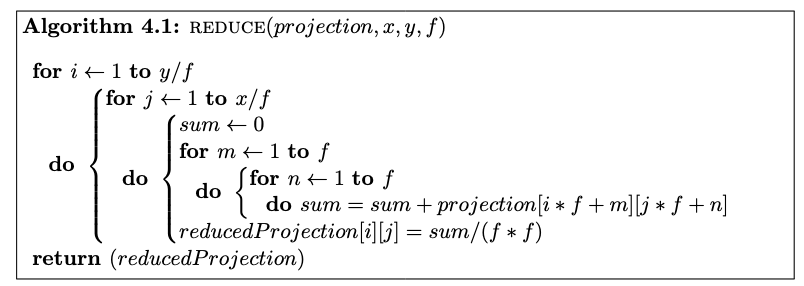
\includegraphics[width=3in]{figures/algorithm.png}

  \caption{\label{fig:fig2}This is my great pseudocode}
  
  \end{figure}





%%%%%%%%%%%%%%%%%%%%%%%%%%%%%%%%%%%%%%%%%%%%%%%%%%%%%%%%%%%%%%%%%%%
%
% Latex float chart example
% Copied from http://www.texample.net/tikz/examples/simple-flow-chart/
%
%%%%%%%%%%%%%%%%%%%%%%%%%%%%%%%%%%%%%%%%%%%%%%%%%%%%%%%%%%%%%%%%%%%

Figure~\ref{fig:fig3} is a sample float chart copy from this website \cite{floatchart}
   
  \begin{figure}[!ht]
 \centering
 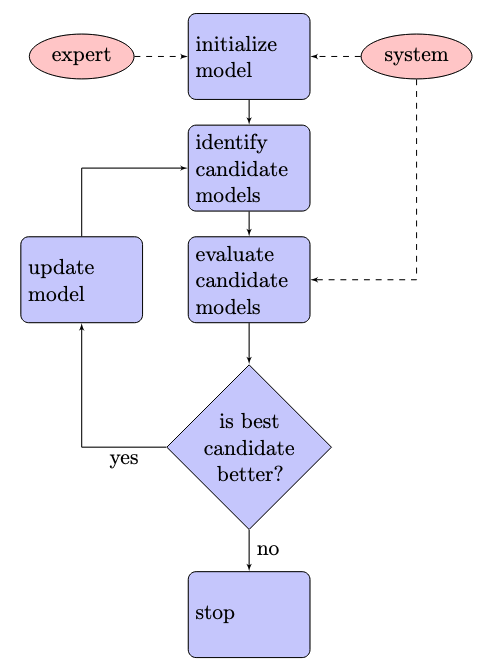
\includegraphics[width=3in]{figures/flowchart.png}

  \caption{\label{fig:fig3}This is my great float chart}
  
  \end{figure}


%%%%%%%%%%%%%%%%%%%%%%%%%%%%%%%%%%%%%%%%%%%%%%%%%%%%%%%%%%%%%%%%%%%

\subsection{Mathematics}

If your project idea needs mathematics to formulate your methods, \LaTeX{} is great at typesetting mathematics. Let $X_1, X_2, \ldots, X_n$ be a sequence of independent and identically distributed random variables with $\text{E}[X_i] = \mu$ and $\text{Var}[X_i] = \sigma^2 < \infty$, and let
$$S_n = \frac{X_1 + X_2 + \cdots + X_n}{n}
      = \frac{1}{n}\sum_{i}^{n} X_i$$
denote their mean. Then as $n$ approaches infinity, the random variables $\sqrt{n}(S_n - \mu)$ converge in distribution to a normal $\mathcal{N}(0, \sigma^2)$.

\section{Implementation Overview}

The implementation of the phishing detection system is structured to integrate data preprocessing, neural network modeling, and training in a modular and scalable manner. Below, we provide a high-level overview of the main components.

\subsection{Custom Dataset Class}
The \texttt{PhishingDataset} class is designed to facilitate data loading and processing. It extends the PyTorch \texttt{Dataset} class and provides methods for retrieving features and labels as tensors. This design ensures seamless compatibility with PyTorch's \texttt{DataLoader}, enabling efficient batch-wise data handling during training and evaluation.

\subsection{Neural Network Architecture}
The phishing detection model is implemented as a feedforward neural network, encapsulated in the \texttt{PhishingNN} class. The network comprises:
\begin{itemize}
    \item An input layer, which maps the feature space to a hidden representation.
    \item Two hidden layers with ReLU activations to introduce non-linearity and enhance the model's capacity to learn complex patterns.
    \item An output layer producing logits for binary classification.
\end{itemize}
The modular design of the network allows for straightforward modifications and experimentation with different architectures.

\subsection{Data Preprocessing and Splitting}
The dataset, containing phishing-related features and labels, is preprocessed using the \texttt{load\_data} function. This includes:
\begin{itemize}
    \item Splitting the data into training and testing subsets using an 80-20 split ratio.
    \item Normalizing features with \texttt{StandardScaler} to improve convergence during training.
\end{itemize}
This preprocessing ensures the input data is well-suited for training the neural network.

\subsection{Dataset and DataLoader Integration}
To streamline data handling, the preprocessed data is encapsulated into instances of \texttt{PhishingDataset}. These are further wrapped in PyTorch \texttt{DataLoader} objects, which provide efficient batch processing and shuffling capabilities. A batch size of 64 is used during training to balance computational efficiency and gradient stability.

\subsection{Model Training}
The training process is implemented in the \texttt{train\_model} function, which integrates all components:
\begin{itemize}
    \item The model is trained using the Adam optimizer with a learning rate of 0.001 and \texttt{CrossEntropyLoss} as the objective function.
    \item A training loop iterates over the data for 15 epochs, performing forward propagation, loss computation, and backpropagation with gradient updates.
    \item The average loss per epoch is logged to monitor the training progress.
    \item Training time is recorded to evaluate the computational efficiency of the pipeline.
\end{itemize}

\subsection{Discussion}
This modular implementation provides a solid foundation for phishing detection using neural networks. The design emphasizes scalability and flexibility, enabling easy modifications for future extensions. Additionally, the implementation tracks loss during training, to visualize model performance during each epoch. In our results section, we discuss the overall performance of the model, as well as any future improvements that could be made.

\section{Testing and Experiments}
In this section, describe your testing and experiment design and setup, and conduct the testing and experiments, and generate data. 

Need to explain why your experiment design will do what is supposed to do, and describe the expected result, and how the result may validate your ideas and/or support your project. 
\section{Data Analysis}

Based on the data generated from the testing and experiments, we derived the following results. The global temperature is increasing at an alarming rate as illustrated in Figure~\ref{fig:fig4}.  It is not real data, it is for demonstration only. 

  \begin{figure}[!ht]
 \centering
 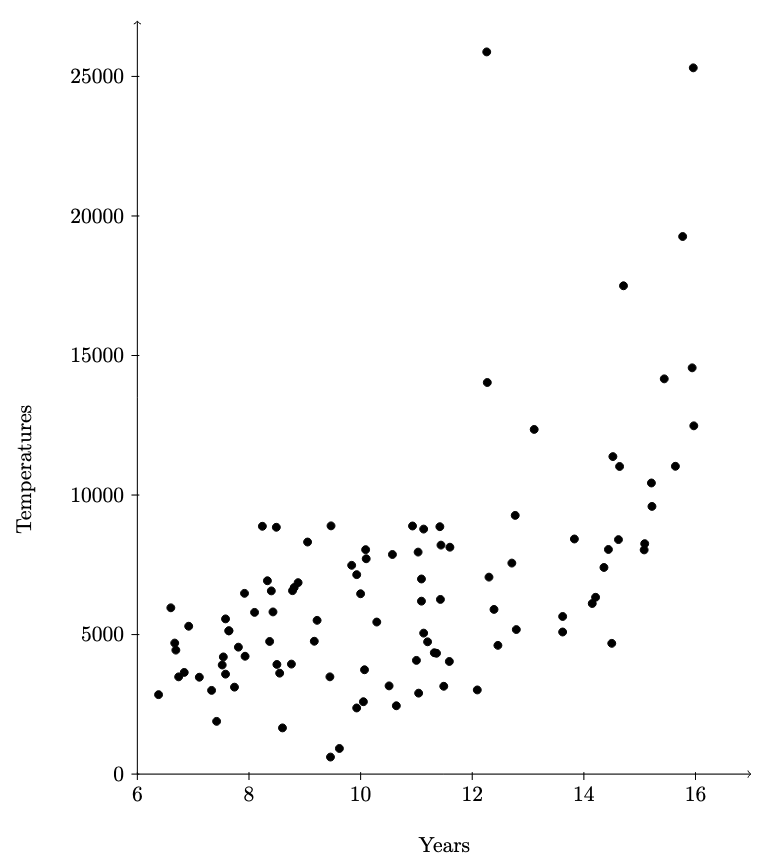
\includegraphics[width=3in]{figures/plot.png}

  \caption{\label{fig:fig4} Recent Global Temperature Data}
  
  \end{figure}
  
\section{Conclusions}
In this section, you should provide a concise summary of your work, and state the importance of your idea and your contribution towards solving the problem. Point out any improvement that could be done if you had more time. List some ideas for future work. 

\section{Acknowledgment}
I thank my advisor for the guidance and I appreciate the financial and emotion support from my family and sponsors, .... 
\bibliographystyle{IEEEtran}
\bibliography{ref} 
\section{Appendices}

This includes all source code, scripts, and any material that helps other people replicate the results. 





% ------------------------------------------------------------------------------
% End document
% ------------------------------------------------------------------------------
\end{document}
